\documentclass[12pt,a4paper]{article}

% ─── Page Layout ───────────────────────────────────────────────────────────────
\usepackage[a4paper, margin=0.8in, headheight=14pt]{geometry}

% ─── Fonts (XeLaTeX) ───────────────────────────────────────────────────────────
\usepackage{fontspec}
\usepackage{unicode-math}
\setmainfont{TeX Gyre Pagella}
\setmonofont[Scale=0.88]{TeX Gyre Cursor}
\setmathfont{Latin Modern Math}

% ─── Packages ──────────────────────────────────────────────────────────────────
\usepackage{xcolor}
\usepackage{colortbl}
\usepackage{titlesec}
\usepackage{enumitem}
\usepackage{tabularx}
\usepackage{booktabs}
\usepackage{array}
\usepackage{amsmath}
\usepackage{tikz}
\usetikzlibrary{shapes.geometric, arrows.meta, positioning, calc, fit, decorations.pathreplacing, patterns}
\usepackage{tcolorbox}
\tcbuselibrary{skins, breakable}
\usepackage{hyperref}
\usepackage{fancyhdr}
\usepackage{graphicx}
\usepackage{microtype}
\hyphenpenalty=10000
\exhyphenpenalty=10000
\sloppy
\usepackage{caption}
\usepackage{setspace}
\usepackage{multirow}
\usepackage{tocloft}

% ─── Q&A helper ────────────────────────────────────────────────────────────────
\newcommand{\Q}[1]{\textbf{#1}\par\noindent\ignorespaces}

% ─── Colour Palette ────────────────────────────────────────────────────────────
\definecolor{myred}{RGB}{196,30,58}
\definecolor{mydark}{RGB}{30,30,50}
\definecolor{mygreen}{RGB}{14,120,80}
\definecolor{myteal}{RGB}{0,130,140}
\definecolor{myamber}{RGB}{180,100,0}
\definecolor{mypurple}{RGB}{100,30,160}
\definecolor{mygray}{RGB}{246,247,249}
\definecolor{mgframe}{RGB}{180,185,200}
\definecolor{watermark}{RGB}{145,150,170}
\definecolor{hdrred}{RGB}{250,232,235}
\definecolor{hdrgreen}{RGB}{220,244,233}
\definecolor{hdrteal}{RGB}{220,242,244}
\definecolor{hdramber}{RGB}{253,242,215}
\definecolor{hdrpurple}{RGB}{238,228,255}
\definecolor{hdrgray}{RGB}{238,240,245}
\definecolor{rowalt}{RGB}{250,251,253}

% ─── Section Formatting ────────────────────────────────────────────────────────
\titleformat{\section}{\large\bfseries\color{myred}}{\thesection.}{0.5em}{}[\vspace{1pt}{\color{myred}\rule{\linewidth}{0.8pt}}]
\titleformat{\subsection}{\normalsize\bfseries\color{myteal}}{\thesubsection}{0.5em}{}
\titlespacing*{\section}{0pt}{18pt}{7pt}
\titlespacing*{\subsection}{0pt}{11pt}{4pt}

% ─── Paragraph ─────────────────────────────────────────────────────────────────
\setlength{\parindent}{0pt}
\setlength{\parskip}{4pt}

% ─── TOC Styling ───────────────────────────────────────────────────────────────
\renewcommand{\cfttoctitlefont}{\large\bfseries\color{myred}}
\renewcommand{\cftaftertoctitle}{\par\noindent{\color{myred}\rule{\linewidth}{0.8pt}}}
\setlength{\cftbeforetoctitleskip}{0pt}
\setlength{\cftaftertoctitleskip}{6pt}
\renewcommand{\cftsecfont}{\normalsize\bfseries\color{mydark}}
\renewcommand{\cftsecpagefont}{\normalsize\bfseries\color{mydark}}
\renewcommand{\cftsecleader}{\cftdotfill{\cftdotsep}}
\setlength{\cftbeforesecskip}{7pt}
\renewcommand{\cftsubsecfont}{\small\color{mydark}}
\renewcommand{\cftsubsecpagefont}{\small\color{mydark}}
\setlength{\cftbeforesubsecskip}{3pt}
\setlength{\cftsubsecindent}{1.4em}

% ─── Table helpers ─────────────────────────────────────────────────────────────
\renewcommand{\arraystretch}{1.45}
\setlength{\tabcolsep}{6pt}
\arrayrulecolor{mydark}
\newcolumntype{B}[1]{>{\small\bfseries\raggedright\arraybackslash}m{#1}}
\newcolumntype{Y}{>{\small\raggedright\arraybackslash}X}
\renewcommand{\tabularxcolumn}[1]{m{#1}}

% ─── Header / Footer ───────────────────────────────────────────────────────────
\pagestyle{fancy}
\fancyhf{}
\fancyhead[L]{\small\color{myred}\textbf{OE-EC803B}\;\color{mydark}--- Big Data Analysis}
\fancyhead[R]{\small\color{myteal}\textbf{Module 4 Notes}}
\fancyfoot[C]{\small\color{mydark}\thepage}
\fancyfoot[R]{\small\color{watermark}\textit{\copyright\ Biraj Sarkar}}
\renewcommand{\headrulewidth}{0.5pt}
\renewcommand{\footrulewidth}{0.3pt}

% ─── Hyperref ──────────────────────────────────────────────────────────────────
\hypersetup{colorlinks=true, linkcolor=myteal, urlcolor=myteal,
  pdfauthor={Biraj Sarkar}, pdftitle={OE-EC803B --- Module 4 Notes}}

% ─── tcolorbox styles ──────────────────────────────────────────────────────────
\tcbset{
  tikzbox/.style={colback=mygray, colframe=mgframe, boxrule=0.6pt, arc=4pt,
    left=8pt, right=8pt, top=6pt, bottom=6pt,
    colbacktitle=mgframe, coltitle=mydark, fonttitle=\small\bfseries, unbreakable},
  defbox/.style={colback=hdrgreen, colframe=mygreen, boxrule=0.8pt, arc=4pt,
    left=9pt, right=9pt, top=6pt, bottom=6pt,
    colbacktitle=mygreen, coltitle=white, fonttitle=\small\bfseries},
  formulabox/.style={colback=hdrteal, colframe=myteal, boxrule=0.8pt, arc=4pt,
    left=9pt, right=9pt, top=7pt, bottom=7pt,
    colbacktitle=myteal, coltitle=white, fonttitle=\small\bfseries},
  examplebox/.style={colback=hdramber, colframe=myamber, boxrule=0.8pt, arc=4pt,
    left=9pt, right=9pt, top=6pt, bottom=6pt,
    colbacktitle=myamber, coltitle=white, fonttitle=\small\bfseries},
  masonbox/.style={colback=hdrpurple, colframe=mypurple, boxrule=0.8pt, arc=4pt,
    left=9pt, right=9pt, top=6pt, bottom=6pt,
    colbacktitle=mypurple, coltitle=white, fonttitle=\small\bfseries},
  exambox/.style={colback=hdrpurple, colframe=mypurple, boxrule=1pt, arc=5pt,
    left=10pt, right=10pt, top=8pt, bottom=8pt,
    colbacktitle=mypurple, coltitle=white, fonttitle=\bfseries,
    breakable, title after break={\textbf{Frequently Asked / Viva Questions (contd.)}}}
}
\tcbset{breakable}

% ─── TikZ styles ───────────────────────────────────────────────────────────────
\tikzset{
  block/.style={rectangle, draw=myteal, fill=hdrteal,
    text width=2.2cm, align=center, minimum height=0.9cm,
    font=\small, rounded corners=3pt, line width=0.7pt},
  redblock/.style={rectangle, draw=myred, fill=hdrred,
    text width=2.2cm, align=center, minimum height=0.9cm,
    font=\small, rounded corners=3pt, line width=0.7pt},
  arrow/.style={-Stealth, thick, color=mydark},
  redarrow/.style={-Stealth, thick, color=myred},
  line/.style={thick, color=mydark}
}

\begin{document}

% ═══════════════════════════════════════════════════════════════════════════════
% TITLE BLOCK
% ═══════════════════════════════════════════════════════════════════════════════
\begin{center}
  \hfill \textit{Exam-Ready Short Notes} \\
  \vspace{6pt}
  {\LARGE\bfseries\color{myred} OE-EC803B --- Big Data Analysis}\\[5pt]
  {\normalsize\color{mydark} Semester VIII \quad$\bullet$\quad 3L:0T:0P \quad$\bullet$\quad 3 Credits}\\[3pt]
  {\normalsize\color{myteal}\textbf{Module 4: Hadoop Ecosystem Components (Pig, Hive, HBase, Big SQL)}}\\[3pt]
  {\small\color{mydark} CGEC \;$|$\; B.Tech ECE (2023--27) \;$|$\; \textit{Biraj Sarkar}}
\end{center}
\vspace{2pt}
\noindent{\color{myred}\rule{\linewidth}{1.5pt}}
\vspace{2pt}

\hypersetup{linkcolor=mydark}
\tableofcontents
\hypersetup{linkcolor=myteal}
\newpage

% ===============================================================================
\section{Apache Pig}
% ===============================================================================

\begin{tcolorbox}[defbox, title={Apache Pig}]
  \textbf{Apache Pig} is a high-level dataflow platform designed for processing large datasets on Hadoop. It provides a procedural dataflow programming language called \textbf{Pig Latin}, which compiles scripts into sequences of MapReduce jobs executed across a YARN cluster.
\end{tcolorbox}

\subsection{Execution Modes and Components}
\begin{itemize}[leftmargin=*, itemsep=3pt]
  \item \textbf{Local Mode:} Runs in a single JVM using the local filesystem. Excellent for testing and debugging.
  \item \textbf{MapReduce Mode:} Translates scripts into MapReduce jobs and executes them on an active Hadoop cluster.
  \item \textbf{Grunt Shell:} The interactive command-line shell used to type Pig Latin statements.
  \item \textbf{UDF (User Defined Functions):} Allows developers to write custom processing logic in Java, Python, or JavaScript when Pig's built-in operators are insufficient.
\end{itemize}

\subsection{Pig Latin Data Model}
Pig Latin supports both simple types (e.g., `int`, `chararray`) and complex nested types:
\begin{itemize}[leftmargin=*, itemsep=3pt]
  \item \textbf{Atom:} Any single value stored as a string (e.g., `'Biraj'`, `45`).
  \item \textbf{Tuple:} An ordered set of fields (e.g., `(Biraj, 22, CGEC)`).
  \item \textbf{Bag:} A collection of tuples (e.g., `{(Biraj, 22), (Amit, 23)}`).
  \item \textbf{Map:} A set of key-value pairs (e.g., \texttt{['name'\#'Biraj', 'age'\#'22']}).
\end{itemize}

\subsection{Core Processing Operators}
\begin{itemize}[leftmargin=*, itemsep=3pt]
  \item `LOAD`: Ingests data from HDFS files.
  \item `FILTER`: Selects tuples from a relation based on conditions.
  \item `FOREACH ... GENERATE`: Transforms data columns.
  \item `GROUP`: Collects tuples sharing a key into a bag.
  \item `JOIN`: Joins relations based on matching keys.
\end{itemize}

% ===============================================================================
\section{Apache Hive}
% ===============================================================================

\begin{tcolorbox}[defbox, title={Apache Hive}]
  \textbf{Apache Hive} is a data warehouse software system built on top of Apache Hadoop that provides data summarization, ad-hoc querying, and analysis of large datasets stored in HDFS. It provides an SQL-like query language called \textbf{HiveQL}.
\end{tcolorbox}

\subsection{Hive Architecture}
Hive translates SQL-like HiveQL statements into MapReduce, Tez, or Spark jobs.

\begin{tcolorbox}[tikzbox, title={Hive System Architecture}]
\centering
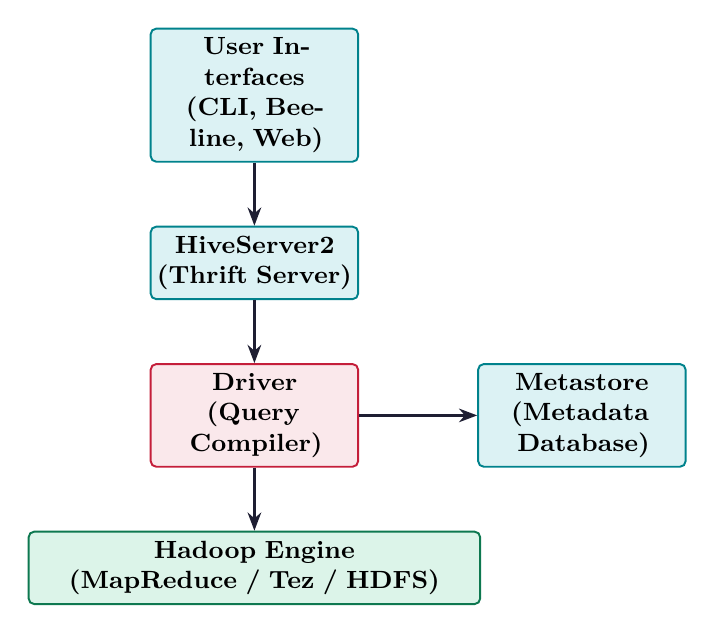
\begin{tikzpicture}[node distance=0.7cm and 1.0cm,
  bblock/.style={rectangle, draw=myteal, fill=hdrteal, text width=2.4cm, align=center, minimum height=0.8cm, font=\small\bfseries, rounded corners=2pt, line width=0.7pt},
  rblock/.style={rectangle, draw=myred, fill=hdrred, text width=2.4cm, align=center, minimum height=0.8cm, font=\small\bfseries, rounded corners=2pt, line width=0.7pt},
  gblock/.style={rectangle, draw=mygreen, fill=hdrgreen, text width=5.5cm, align=center, minimum height=0.75cm, font=\small\bfseries, rounded corners=2pt, line width=0.7pt}]

  % Nodes
  \node[bblock] (ui) {User Interfaces\\(CLI, Beeline, Web)};
  \node[bblock, below=0.8cm of ui] (hs2) {HiveServer2\\(Thrift Server)};

  \node[rblock, below=0.8cm of hs2] (driver) {Driver\\(Query Compiler)};
  \node[bblock, right=1.5cm of driver] (ms) {Metastore\\(Metadata Database)};
  \node[gblock, below=0.8cm of driver] (hadoop) {Hadoop Engine\\(MapReduce / Tez / HDFS)};

  % Arrows
  \draw[arrow] (ui) -- (hs2);
  \draw[arrow] (hs2) -- (driver);
  \draw[arrow] (driver) -- (ms);
  \draw[arrow] (driver) -- (hadoop);

\end{tikzpicture}
\end{tcolorbox}

\begin{itemize}[leftmargin=*, itemsep=3pt]
  \item \textbf{Metastore:} A relational database (typically MySQL or Derby) that stores schema definitions, column details, and partition metadata.
  \item \textbf{HiveServer2:} The execution endpoint allowing remote JDBC/ODBC clients to submit queries.
\end{itemize}

\subsection{Managed vs. External Tables}
Hive supports two types of tables to control data ownership:

\par\vspace{6pt}\noindent
{\renewcommand{\arraystretch}{1.4}%
\begin{tabularx}{\linewidth}{|B{3.2cm}|Y|Y|}
\hline
\textbf{Feature} & \textbf{Managed Table (Internal)} & \textbf{External Table} \\
\hline
Data Ownership & Hive owns both the metadata and the data. & Hive only owns the metadata. \\
\hline
Storage Path & Default directory: `/user/hive/warehouse/` & User-defined HDFS location. \\
\hline
`DROP TABLE` Impact & Deletes both the HDFS data and metadata. & Deletes metadata; HDFS data remains intact. \\
\hline
Use Case & Temporary tables, internal application data. & Sharing datasets with Spark, Pig, or MapReduce. \\
\hline
\end{tabularx}}

\subsection{Partitioning vs. Bucketing}
Hive optimizes query performance using two layout patterns:

\begin{tcolorbox}[formulabox, title={Partitioning vs. Bucketing Properties}]
  \begin{itemize}[leftmargin=*, noitemsep]
    \item \textbf{Partitioning:} Divides a table into subdirectories based on column values (e.g., `/country=IN/`, `/country=US/`). It significantly reduces query search space by pruning directories.
    \item \textbf{Bucketing:} Distributes table rows into a fixed number of files (buckets) based on a hash function of a column (e.g., `hash(userID) \% numBuckets`). It speeds up joins and sampling on high-cardinality columns.
  \end{itemize}
\end{tcolorbox}

% ===============================================================================
\section{Apache HBase}
% ===============================================================================

\begin{tcolorbox}[defbox, title={Apache HBase}]
  \textbf{Apache HBase} is a distributed, column-oriented, multi-dimensional, NoSQL database built on top of HDFS, modeled after Google's Bigtable, designed to provide random, real-time read/write access to billions of rows and columns.
\end{tcolorbox}

\subsection{HBase Architecture and Components}
HBase achieves horizontal scale using master-slave coordinators:
\begin{itemize}[leftmargin=*, itemsep=3pt]
  \item \textbf{HMaster:} Coordinates the cluster, assigns regions to RegionServers, and handles schema updates.
  \item \textbf{RegionServer:} Manages a set of dynamic table splits called \textbf{Regions}. Handles client read/write requests directly.
  \item \textbf{Write-Ahead Log (WAL):} A local disk file where writes are written first for durability before committing to RAM.
  \item \textbf{MemStore:} The write buffer in RAM. Writes are accumulated here first.
  \item \textbf{HFile:} The physical file format stored on HDFS. When a MemStore fills up (flushes), its contents are written to disk as an HFile.
\end{itemize}

\begin{tcolorbox}[tikzbox, title={HBase Architecture}]
\centering
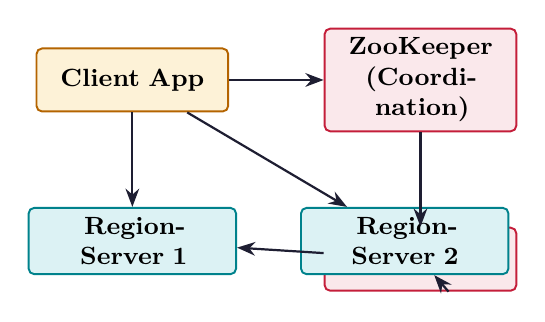
\begin{tikzpicture}[node distance=0.7cm and 0.8cm,
  mblock/.style={rectangle, draw=myred, fill=hdrred, text width=2.2cm, align=center, minimum height=0.8cm, font=\small\bfseries, rounded corners=2pt, line width=0.7pt},
  rblock/.style={rectangle, draw=myteal, fill=hdrteal, text width=2.4cm, align=center, minimum height=0.8cm, font=\small\bfseries, rounded corners=2pt, line width=0.7pt},
  cblock/.style={rectangle, draw=myamber, fill=hdramber, text width=2.2cm, align=center, minimum height=0.8cm, font=\small\bfseries, rounded corners=2pt, line width=0.7pt},
  bgbox/.style={draw=mgframe, fill=mygray, line width=0.8pt, rounded corners=4pt, inner sep=6pt}]

  % Nodes
  \node[cblock] (client) {Client App};
  \node[mblock, right=1.2cm of client] (zk) {ZooKeeper\\(Coordination)};
  \node[mblock, below=1.2cm of zk] (hm) {HMaster};

  \node[rblock, below=1.2cm of client] (rs1) {RegionServer 1};
  \node[rblock, right=0.8cm of rs1] (rs2) {RegionServer 2};

  % Connections
  \draw[arrow] (client) -- (zk);
  \draw[arrow] (zk) -- (hm);
  \draw[arrow] (client) -- (rs1);
  \draw[arrow] (client) -- (rs2);
  \draw[arrow] (hm) -- (rs1);
  \draw[arrow] (hm) -- (rs2);

\end{tikzpicture}
\end{tcolorbox}

% ===============================================================================
\section{IBM Big SQL}
% ===============================================================================

\begin{tcolorbox}[defbox, title={IBM Big SQL}]
  \textbf{IBM Big SQL} is an enterprise-grade, SQL-on-Hadoop engine that provides an ANSI-SQL compliant query compiler and Massively Parallel Processing (MPP) execution framework to query data stored across HDFS, Hive, and HBase directly.
\end{tcolorbox}

Big SQL utilizes a shared-nothing MPP architecture that executes SQL queries natively on Hadoop data blocks without the latency overhead of MapReduce translations, supporting complex joins and standard business intelligence integrations.

\newpage

% ═══════════════════════════════════════════════════════════════════════════════
% QUICK REVISION PAGE
% ═══════════════════════════════════════════════════════════════════════════════
\begin{center}
  {\large\bfseries\color{myred} Quick Revision --- Module 4}\\[3pt]
  {\small\color{mydark} Pig Latin, HiveQL, HBase NoSQL \& Big SQL $|$ OE-EC803B}
\end{center}
\noindent{\color{myred}\rule{\linewidth}{1.2pt}}
\vspace{8pt}

\begin{tcolorbox}[defbox, title={\textbf{One-Line Definitions}}]
\begin{itemize}[leftmargin=*, itemsep=3pt, topsep=0pt]
  \item \textbf{Pig Latin:} A high-level dataflow programming language used to describe data transformation pipelines.
  \item \textbf{HiveQL:} An SQL-like query language that is compiled into execution plans (like Tez or MapReduce).
  \item \textbf{Metastore:} The repository that stores structural metadata and schema information for Hive tables.
  \item \textbf{RegionServer:} An HBase slave node that serves read and write operations for a subset of row keys.
  \item \textbf{Big SQL:} An enterprise Massively Parallel Processing (MPP) SQL querying engine for Hadoop clusters.
\end{itemize}
\end{tcolorbox}

\vspace{6pt}

\begin{tcolorbox}[exambox, title={\textbf{Frequently Asked / Viva Questions}}]
\begin{enumerate}[leftmargin=*, topsep=0pt, label=\textbf{Q\arabic*.}, itemsep=5pt]
  \item \Q{Compare Apache Pig and Apache Hive.}
        Apache Pig uses a procedural dataflow scripting language (Pig Latin) suited for ETL pipelines and data engineers. Apache Hive uses a declarative SQL-like language (HiveQL) suited for data warehousing and business intelligence.
        
  \item \Q{What happens to the HDFS data when a Managed Table vs. an External Table is dropped in Hive?}
        Dropping a Managed Table deletes both the table metadata and the physical data files in HDFS. Dropping an External Table deletes only the Hive schema metadata, leaving the physical data files intact in HDFS.
        
  \item \Q{Explain the difference between Partitioning and Bucketing in Hive.}
        Partitioning organizes data into separate subdirectories based on column values (pruning queries). Bucketing splits data into a fixed number of files based on a hash of a column, which optimizes joins on high-cardinality columns.
        
  \item \Q{Detail the write path of a record in Apache HBase.}
        A client write is first appended to the Write-Ahead Log (WAL) on disk for durability, then written to the in-memory \textbf{MemStore} in RAM. Once the write is in MemStore, the client receives an ACK.
        
  \item \Q{When does HBase flush data, and what file format is generated?}
        When the in-memory MemStore reaches its capacity threshold (typically 128MB), HBase flushes its sorted key-value contents to HDFS, creating a new binary \textbf{HFile}.
        
  \item \Q{Why is HBase called a Column-Family NoSQL database?}
        HBase groups columns together into \textbf{Column Families} (defined during table creation). Internally, columns belonging to the same column family are stored in the same physical HFile, optimizing access for selective queries.
        
  \item \Q{What are the complex nested data types supported in Pig Latin?}
        \textbf{Tuple} (an ordered list of fields), \textbf{Bag} (an unordered collection of tuples), and \textbf{Map} (a set of key-value pairs).
        
  \item \Q{Explain the role of ZooKeeper in an HBase cluster.}
        ZooKeeper coordinates Region assignment, detects RegionServer failures, maintains the root table location, and prevents active-standby conflicts by coordinating HMaster elections.
        
  \item \Q{What are UDF, UDAF, and UDTF in Hive?}
        \begin{itemize}[leftmargin=*, noitemsep]
          \item \textbf{UDF:} User Defined Function (maps 1 row to 1 output).
          \item \textbf{UDAF:} User Defined Aggregate Function (maps multiple rows to 1 aggregated output).
          \item \textbf{UDTF:} User Defined Table Generating Function (maps 1 row to multiple output rows/tables).
        \end{itemize}
        
  \item \Q{Describe the execution flow of a Big SQL query.}
        Big SQL bypasses MapReduce. The Big SQL coordinator compiles SQL queries, optimizes execution plans, and uses an MPP engine to distribute query processing fragments directly to local nodes containing target HDFS blocks.
\end{enumerate}
\end{tcolorbox}

\vspace{6pt}

\begin{tcolorbox}[tikzbox, title={\textbf{Comparison Snapshot}}]
\textbf{Traditional RDBMS vs. NoSQL HBase:}\par\vspace{6pt}\noindent
{\renewcommand{\arraystretch}{1.4}%
\begin{tabularx}{\linewidth}{|B{3.2cm}|Y|Y|}
\hline
\textbf{Feature} & \textbf{Traditional RDBMS} & \textbf{NoSQL HBase} \\
\hline
Data Layout & Row-oriented (stores entire row together) & Column-family oriented (stores family columns together) \\
\hline
Schema Flexibility & Schema-on-write (rigid definitions) & Schema-less (columns can be added dynamically) \\
\hline
Transaction Support & Full ACID transactions across multiple tables & ACID transactions supported at Row-level only \\
\hline
Scaling Pattern & Vertical (bigger machines) & Horizontal (adding RegionServers in parallel) \\
\hline
Join Support & Rich declarative SQL joins & No native join support (requires MapReduce/Spark) \\
\hline
Null Value Storage & Consumes space for NULL definitions & Zero storage overhead for empty cells (sparse tables) \\
\hline
\end{tabularx}}
\end{tcolorbox}

\end{document}
